\documentclass[12pt, letterpaper, titlepage]{article}
\usepackage{graphicx}
\usepackage{hyperref}
\usepackage[margin=1in]{geometry}
\usepackage{natbib}
\usepackage{cleveref}
%\DeclareMathOperator*{\argmax}{arg\,max}
\hypersetup{colorlinks = true, linkcolor = blue, citecolor=blue, urlcolor = blue}

\title{CSE 5825: Project 3}
\author{Owen Fiore and Jared Sullivan}

\begin{document}
\maketitle

\section{Abstract}
We set out to find a lower dimensional space that characterizes each NBA player’s play style.  An autoencoder was built to transform the high dimensional player data to a numerical vector representing a player’s play style.  Doing this we were able to visualize the output and test our latent space with known truths from the NBA.  While player position and play style are not always expected to be correlated, what we found re-assured us that the autoencoder worked effectively.  After verifying the latent space we clustered on it using a Gaussian mixture model and used these results to draw assumptions about the types of players in each cluster.  Additionally, we were able to track trends in play styles over the years to see how demand for different position archetypes has changed over time to try and measure how much the NBA has changed from 2000 to 2023.
\section{Introduction}
In the NBA, each team is allowed five players on the court at one time, typically with one for each position: point guard, shooting guard, small forward, power forward, and center.  However, players such as LeBron James do not always fit nicely into these roles, and can adapt to play whatever their team needs. James has been listed at point guard, shooting guard, small forward, and power forward at various points in his career depending on the surrounding roster  Additionally it is possible for players within the same position to have different play styles such as point guards Steph Curry and Ja Morant.  The contrast between these players is best visualized by a shot chart that shows where each player shoots from.  We see that Curry is an excellent volume outside shooter, attempting many shot attempts behind the three point line and shooting above the league average on those attempts.  To contrast, Morant takes a majority of his shots in the paint, which is unusual for a point guard as the area near the basket is typically defended by larger opponents who are capable of blocking shots from smaller players like Morant.  Morant and Curry are both responsible for being the point guard for their team, but the way they approach their role differs greatly.  We are going to investigate these differences and see if we can better understand whether certain archetypes exist both across and within positions.

We look at many player statistics in the paper, with some of the most notable being shooting percentages (three point, two point, and free throw), rebounds, assists, steals, blocks, turnovers, average shot distance, and salary. These statistics aim to cover all facets of a player’s style and demonstrate their uniqueness and also importantly cover both offensive and defensive statistics.  Identifying players based on how they play basketball can be used to help NBA general managers (who are responsible for constructing their respective team’s roster) identify the types of players that they think can benefit their team.  This can lead to deeper understanding of hidden factors that can contribute to championship success.  General managers are commonly tasked with finding replacements for departing players who either retire, leave in free agency, or request a trade.  If there was a way to represent players as numerical vectors, general managers could search for similar players to try and replace the leaving player. After we have learned representations of the players, we can also cluster them using a Gaussian mixture model.  Clustering will allow us to compare the statistics from each cluster so that we can identify common characteristics within a cluster and use what we know about the NBA to understand the types of players found in each cluster. 

\section{Related Works}
The idea of clustering NBA players using a variety of methods has been researched by other authors who have developed various methodologies to try and cluster NBA players and gain deeper insights from player statistics. \citet{muniz2022weighted} used Principal Components Analysis to shrink and classify NBA statistics themselves into several categories such as offense, defense, rebounding, etc. and then implemented k-means to cluster players into roles. Other papers such as from \citet{guan2023nba2vec} generated results by using natural language processing and neural networks to embed play by play data to predict the outcome of plays depending on the players on the court.  We propose the combination of these methods to build an auto-encoder that is capable of representing players on a lower dimension based on their statistics for the season.  This auto-encoder will learn the representation of players to simplify high dimensional data so that it can be visualized and also understood.


Numerous other papers have applied classification and clustering techniques to group NBA players on a variety of different metrics. K means has proven to be an effective technique to cluster NBA guards, which make up two of the five positions that this paper will attempt to cover \citep{zhang2016application}.  \citet{chi3mixed} also implemented a k means algorithm to try and group players into one of three tiers:key players, bench players, and supporting players with key players being the most impactful to team success. Another interesting approach was undertaken by \citet{wu2018classification} which first manually clustered player based on salary, and then used a k nearest neighbors algorithm to predict how much a player could expect to make in free agency.  This idea of including salary was something that we thought was interesting and very important for actual effectiveness.  Additionally, we thought that while the Principal Component Analysis based techniques employed by \citet{muniz2022weighted} \citet{richardson2019evolution} were interesting, we decided to not use a PCA due to concerns about interpretability and information loss.
One method that we thought was interesting and impactful, was the use of a word embedding model to learn player representations based on play by play data \citep{guan2023nba2vec}.  This paper followed up on a previous one that had used neural networks to encode player shooting tendencies \citep{wang2016classifying}.  However, unlike in the previous two papers, our data source was in the form of player statistics which may be calculated on a per game, season, or 100 possession basis.  Additionally, key differences between this paper and \citet{guan2023nba2vec} is the use of salary to inform both the model and analysis, as well as the use of a Gaussian mixture model to cluster players as an alternative to the k means methods mentioned above. The contribution of this paper is thus to use both autoencoder and Gaussian mixture model techniques to learn, analyze, and most importantly understand the representation of  NBA players from 2000 to 2023 \citep{GMM}.


\section{Methods}
\subsection{Data Cleaning}
Our data comes from Basketball Reference, which is frequently used by many in the basketball analytics community for its in-depth and broad range of data covering players and teams.  From Basketball Reference we pulled various statistics related to a player’s play style for a particular season.  We used every feature that we thought would be important in distinguishing types of players, such as three point shots made per game and three point shooting percentage, as shooting threes can be used to separate all types of players, from guards to centers. Metrics such as rebounding help point towards the physicality of the player, and defensive statistics such as steals and blocks are also very important to include.  One of the more unique statistics is usage rate, which is measure of the percentage of a team’s possessions that result in that player shooting, getting fouled, or turning the ball over.  It is a measure of offensive impact, as we expect strong players to take more shots and have the offense rely on them more to create points.  In addition, we created the feature called \texttt{TruePos} which is the player’s true position and is scaled from 1.00 (all the player’s minutes in a season are at point guard) to 5.00 (all the player’s minutes in a season are at center) as a comparison method against what we actually find using the autoencoder. Note that we did not include the true position as a variable in the auto-encoder.

We decided to remove the players who didn’t play at least 10 games in the season, as that would indicate they were either injured or not a strong enough player to warrant them playing. To use our data on any model we normalized it so that larger sized features don’t exert a greater influence on the model.  For this we decided to use min-max scaling as it guarantees our points will lie between zero and one \citep{scikit-learn}.

\subsection{Embedded Player Model}

The main contribution of this article is the usage of an autoencoder to learn numerical representations on a lower dimension. Unlike other autoencoder models that encode images into a latent space and then reconstruct them, the purpose of the autoencoder is to numerically encode play styles. This is done by using a dense layer to take 41 features and encode them in a two-dimensional space \citep{tensorflow2015-whitepaper}. We know that the model worked well as the mean squared error loss after 40 epochs was only 0.02. Nonetheless, once in the lower dimensional space we will validate our model by taking known truths about NBA players’ play styles and comparing to their representation, for example, making sure a consistent player is represented similarly in consecutive years.  
We decided to use clustering on our embedded space and based on the clustering outcomes from \citet{muniz2022weighted} we decided to set our cluster size to ten.  We used a Gaussian mixture model for clustering in order to gain deeper insights to the types of players that are close together in the latent space.


\section{Results}

\begin{figure}
  \centering
%%%%%%%%%%%%%%%%%%%%%%%%%%%%%%%%%%%%%%
  \begin{minipage}[b]{0.35\textwidth}
    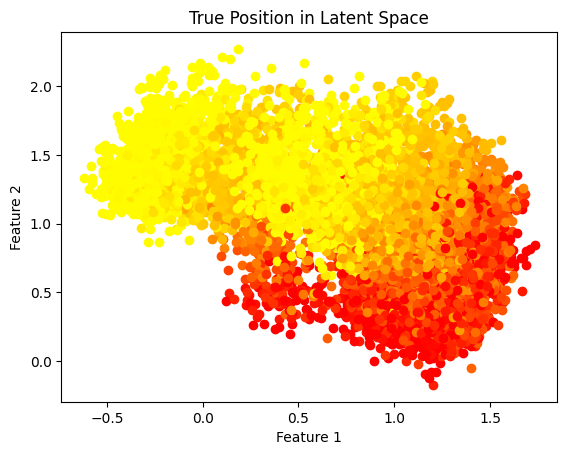
\includegraphics[width=\linewidth]{linearcombo}
    \label{fig:linearcombo}
  \end{minipage}
  \hfill
  \begin{minipage}[b]{0.5\textwidth}
    This graph shows the position of players as a color in the latent space. Red points indicate players whose true position is point guard, orange points are representative of forward, and centers are shown in yellow.  Forwards are often dynamic players and may have different roles on a team which is why it is reasonable for there to be orange points in the red sections as well as in the yellow sections.  Thus our results seem to perform reasonably well given what we know about how positions work in basketball.
  \end{minipage}

  \vspace{1em} % Add some vertical space between images and explanations

%%%%%%%%%%%%%%%%%%%%%%%%%%%%%%%%%%%%%%%

  \begin{minipage}[b]{0.35\textwidth}
    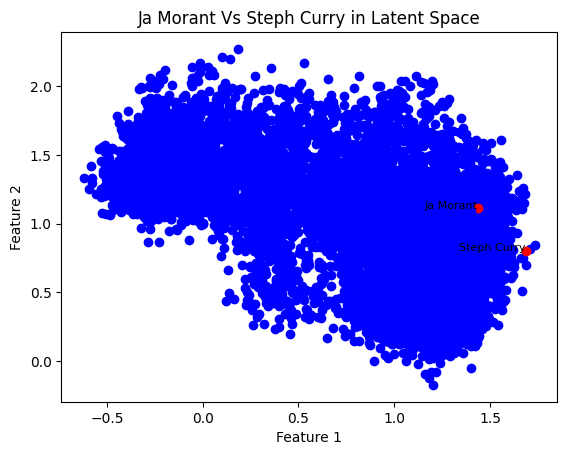
\includegraphics[width=\linewidth]{morantcurry}
    \label{fig:morantcurry}
  \end{minipage}
  \hfill
  \begin{minipage}[b]{0.5\textwidth}
    Here we can see Ja Morant and Steph Curry in the 2023 season.  Ja Morant and Steph Curry both play the same positions, however, they are known for very different styles of play. This can be shown in the latent space as they both lie in a similar zone of player but have significant distance between them showing their differences as well.
  \end{minipage}


  %%%%%%%%%%%%%%%%%%%%%%%%%%%%%%%%%

  \vspace{1em}
  \begin{minipage}[b]{0.35\textwidth}
    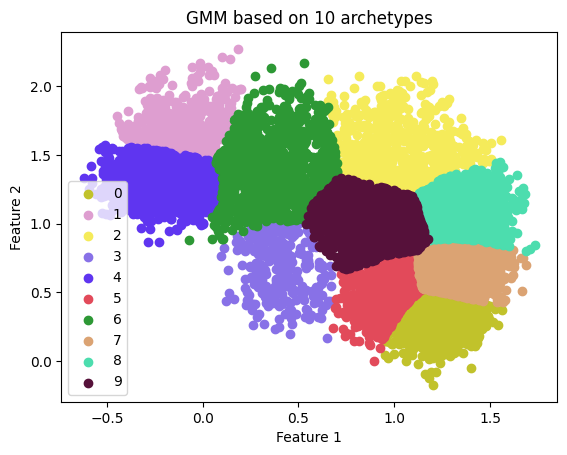
\includegraphics[width=\linewidth]{GaussianMM}
    \label{fig:GaussianMM}
  \end{minipage}
  \hfill
  \begin{minipage}[b]{0.5\textwidth}
    Here is the Gaussian mixture model clustering for the player embedded space.  This graph was very similar to the one generated by using k-means although there were slight variations in how some players were assigned.   
  \end{minipage}

   %%%%%%%%%%%%%%%%%%%%%%%%%%%%%%%%%

  \vspace{1em}
  \begin{minipage}[b]{0.4\textwidth}
    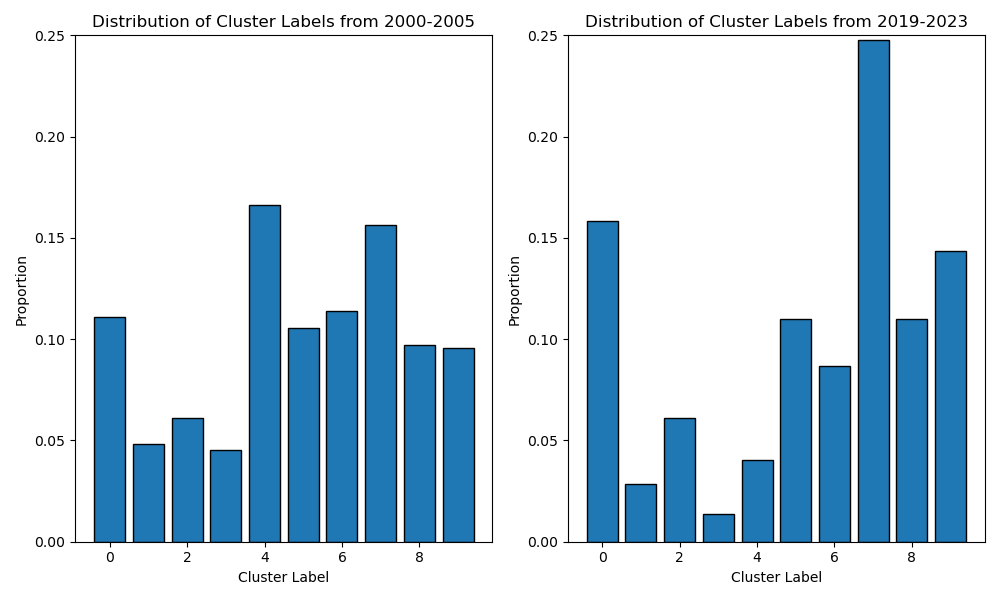
\includegraphics[width=\linewidth]{ClusterCountsByYear}
    \label{ClusterCountsByYear}
  \end{minipage}
  \hfill
  \begin{minipage}[b]{0.5\textwidth}
    The graph above shows the distribution of cluster labels from the five oldest years and five most recent years in the data.  We see that clusters one and four both experienced decreases while clusters seven increased dramatically and clusters zero and nine had large increases.
  \end{minipage}

\end{figure}

\begin{tabular}{ccccccccccc}
    \label{tab:ClusterStats}
    \textbf{label} & \textbf{3P\%} & \textbf{DRB} & \textbf{ORB} & \textbf{AST} & \textbf{STL} & \textbf{BLK} & \textbf{TOV} & \textbf{PTS} & \textbf{USG\%} & \textbf{Dist.} \\
    \hline
    0 & 0.35 & 1.42 & 0.28 & 1.94 & 0.55 & 0.12 & 0.88 & 5.89 & 17.24 & 17.64 \\
    1 & 0.01 & 5.62 & 2.77 & 1.27 & 0.66 & 1.37 & 1.55 & 10.61 & 17.95 & 4.75 \\
    2 & 0.32 & 5.96 & 2.08 & 2.73 & 0.94 & 0.97 & 2.07 & 17.00 & 23.83 & 10.42 \\
    3 & 0.11 & 1.02 & 0.40 & 1.06 & 0.38 & 0.13 & 0.58 & 2.68 & 16.25 & 11.54 \\
    4 & 0.01 & 2.12 & 1.17 & 0.46 & 0.31 & 0.55 & 0.66 & 3.72 & 15.06 & 5.85 \\
    5 & 0.29 & 1.36 & 0.42 & 1.50 & 0.48 & 0.15 & 0.81 & 4.49 & 17.43 & 13.58 \\
    6 & 0.20 & 3.72 & 1.79 & 1.13 & 0.55 & 0.71 & 1.16 & 8.25 & 18.50 & 7.95 \\
    7 & 0.36 & 2.64 & 0.59 & 3.11 & 0.92 & 0.27 & 1.52 & 11.48 & 19.66 & 15.66 \\
    8 & 0.35 & 4.17 & 1.09 & 3.57 & 1.15 & 0.47 & 2.15 & 17.32 & 23.66 & 13.68 \\
    9 & 0.32 & 2.57 & 0.97 & 1.20 & 0.57 & 0.41 & 0.91 & 6.59 & 17.64 & 12.18 \\
    \end{tabular}

 We can compare important statistics for each cluster to determine differences between each cluster (Table~\ref{tab:ClusterStats}).  Some defining characteristics are that clusters zero, seven and eight are made up of very strong perimeter shooters, clusters one and two are made up of skilled forwards and centers who are strong players, whereas clusters three, four and five are made up of weaker ones. Morant is in cluster eight, but is close to cluster two (skilled big men), indicating that Morant's play style is closer to big men than a player like Steph Curry.
\section{Discussion}



Our methods were able to come up with an accurate lower dimension space in which play style and archetypes can be analyzed.  Using this latent space we can pull out features that allow us to characterize a hidden variable that can be useful for many applications.  We considered a number of possible applications related to this work, including models to predict team rating from player rating, models to evaluate team Elo, and models to try and build competitive and cost-effective combinations of players.  

Some limitations of our project are not being able to create a model that can predict the performance of a team based on its players play styles. The idea of team representations becomes more complicated as team statistics are derived from the strength of the players and how much each player plays.  Thus, there are team level statistics that are the result of player statistics.  Nonetheless, this could be used to evaluate the successfulness of team compositions as well as potentially simulate the results between two imaginary teams.  It would be interesting to identify combinations of archetypes that work well together so that general managers can seek out players who would have good chemistry.
\bibliographystyle{chicago}
\bibliography{citations}

\section{Appendix}

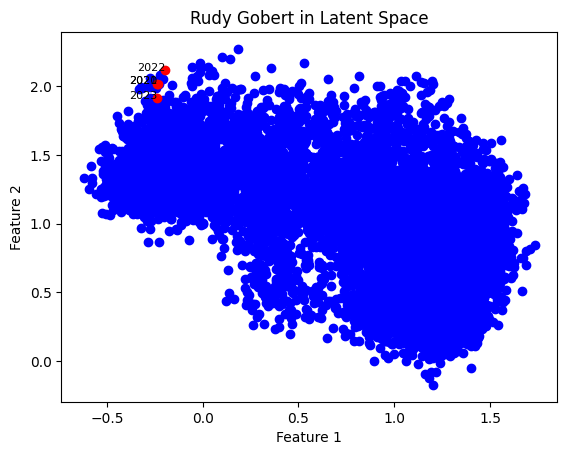
\includegraphics{Gobert}

Rudy Gobert, known for being a defensive anchor on his team, has been one of the most consistent players in the NBA.  From 2020 to 2023 his player representation was extremely constant, granting validity to the autoencoder.

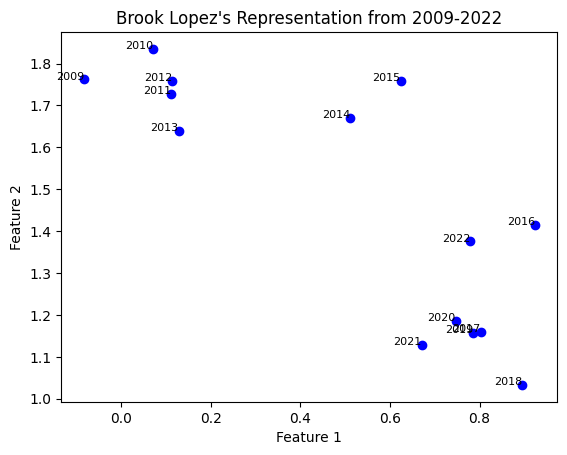
\includegraphics{Lopez}

To contrast Rudy Gobert, Brook Lopez's play-style has evolved over time, with many NBA commentators frequently bringing up how he has expanded his game.  This known characteristic of Lopez is reflected well in his player representation from 2009 to 2023.

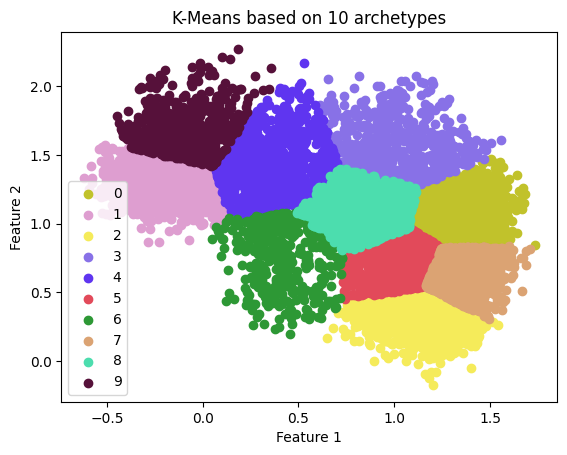
\includegraphics{kmeans}

In addition to using a Gaussian mixture model, we also implemented k means.  The results were generally very similar.


\end{document}